\documentclass[a4paper,UTF8]{article}
\usepackage{ctex}
\usepackage[margin=1.25in]{geometry}
\usepackage{color}
\usepackage{graphicx}
\usepackage{amssymb}
\usepackage{amsmath}
\usepackage{amsthm}
\usepackage{enumerate}
\usepackage{bm}
\usepackage{hyperref}
\usepackage{epsfig}
\usepackage{color}
\usepackage{mdframed}
\usepackage{lipsum}
\usepackage{mathtools}
\usepackage{hyperref}
\usepackage{diagbox}
\usepackage{float}
\usepackage{caption}
\usepackage{algorithm}
\usepackage{algorithmicx}  
\usepackage{algpseudocode}
\usepackage{amsmath} 
\usepackage{graphicx}
\usepackage{subfigure}
\newmdtheoremenv{thm-box}{myThm}
\newmdtheoremenv{prop-box}{Proposition}
\newmdtheoremenv{def-box}{定义}
\usepackage{listings}
\usepackage{xcolor}
\lstset{
	numbers=left, 
	numberstyle= \tiny, 
	keywordstyle= \color{ blue!70},
	commentstyle= \color{red!50!green!50!blue!50}, 
	frame=shadowbox, % 阴影效果
	rulesepcolor= \color{ red!20!green!20!blue!20} ,
	escapeinside=``, % 英文分号中可写入中文
	xleftmargin=2em,xrightmargin=2em, aboveskip=1em,
	framexleftmargin=2em
} 

\usepackage{booktabs}

\setlength{\evensidemargin}{.25in}
\setlength{\textwidth}{6in}
\setlength{\topmargin}{-0.5in}
\setlength{\topmargin}{-0.5in}

% \setlength{\textheight}{9.5in}
%%%%%%%%%%%%%%%%%%此处用于设置页眉页脚%%%%%%%%%%%%%%%%%%
\usepackage{fancyhdr}                                
\usepackage{lastpage}                                           
\usepackage{layout}                                             
\footskip = 10pt 
\pagestyle{fancy}                    % 设置页眉                 
\lhead{研一下学期}                    
\chead{论文阅读笔记}                                                
% \rhead{第\thepage/\pageref{LastPage}页} 
\rhead{Step5}                                                                                               
\cfoot{\thepage}                                                
\renewcommand{\headrulewidth}{1pt}  			%页眉线宽,设为0可以去页眉线
\setlength{\skip\footins}{0.5cm}    			%脚注与正文的距离           
\renewcommand{\footrulewidth}{0pt}  			%页脚线宽,设为0可以去页脚线

\makeatletter 									%设置双线页眉                                        
\def\headrule{{\if@fancyplain\let\headrulewidth\plainheadrulewidth\fi%
\hrule\@height 1.0pt \@width\headwidth\vskip1pt	%上面线为1pt粗  
\hrule\@height 0.5pt\@width\headwidth  			%下面0.5pt粗            
\vskip-2\headrulewidth\vskip-1pt}      			%两条线的距离1pt        
 \vspace{6mm}}     								%双线与下面正文之间的垂直间距              
\makeatother  

%%%%%%%%%%%%%%%%%%%%%%%%%%%%%%%%%%%%%%%%%%%%%%
\numberwithin{equation}{section}
%\usepackage[thmmarks, amsmath, thref]{ntheorem}
\newtheorem{theorem}{Theorem}
\newtheorem*{definition}{Definition}
\newtheorem*{solution}{Solution}
\newtheorem*{prove}{Proof}
\newcommand{\indep}{\rotatebox[origin=c]{90}{$\models$}}

\usepackage{multirow}

%--

%--
\begin{document}
\title{论文阅读笔记\\
Step5}
\author{MF1833063, 史鹏, spwannasing@gmail.com}
\maketitle

\newpage
\section{ERNIE:Enhanced Language Representation with Informative Entities}
此文章是对bert的一次扩展,提出了知识图谱中的多信息实体(informative entity)可以作为外部知识改善语言表征。
\begin{figure}[H]
	\centering
	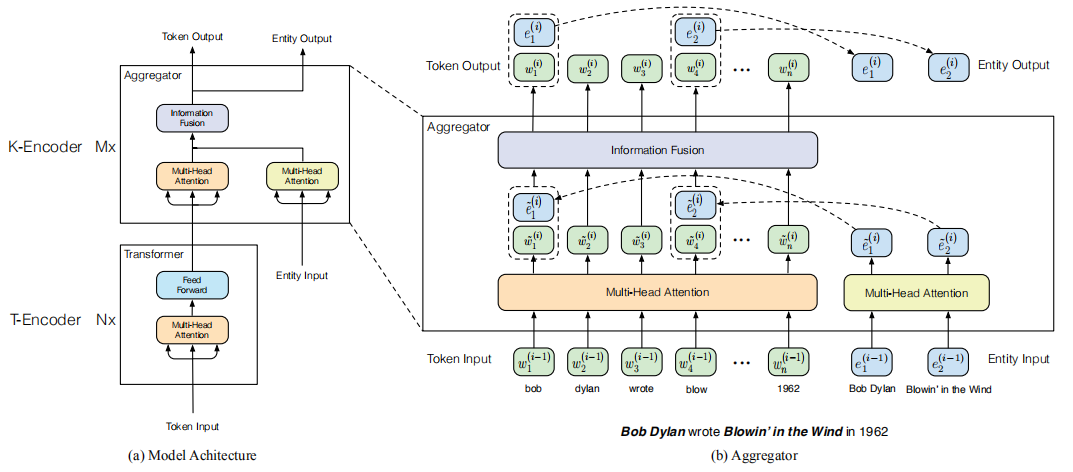
\includegraphics[width=\textwidth]{1-1.png}
	\caption{overview}
\end{figure}
\begin{figure}[H]
	\centering
	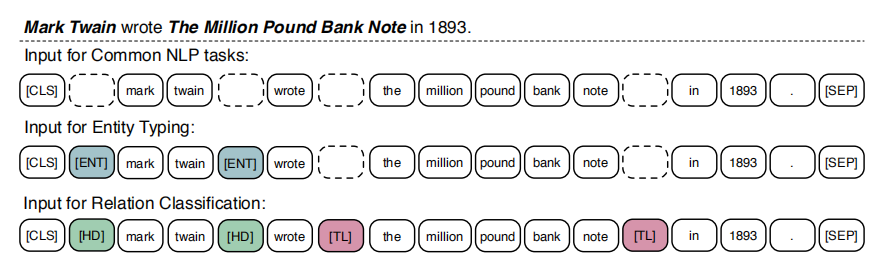
\includegraphics[width=\textwidth]{1-2.png}
	\caption{finetune}
\end{figure}
Knowledgeable Encoder:
\begin{equation}
	\left\{\tilde{\boldsymbol{w}}_{1}^{(i)}, \ldots, \tilde{\boldsymbol{w}}_{n}^{(i)}\right\}=\mathrm{MH}-\mathrm{A} \mathrm{T} \mathrm{T}\left(\left\{\boldsymbol{w}_{1}^{(i-1)}, \ldots, \boldsymbol{w}_{n}^{(i-1)}\right\}\right)
	\end{equation}
	\begin{equation}
		\left\{\tilde{e}_{1}^{(i)}, \ldots, \tilde{e}_{m}^{(i)}\right\}=\operatorname{MH}-\operatorname{ATT}\left(\left\{e_{1}^{(i-1)}, \ldots, e_{m}^{(i-1)}\right\}\right)
		\end{equation}

对于和entity对齐的token:
\begin{equation}
\begin{aligned} \boldsymbol{h}_{j} &=\sigma\left(\tilde{\boldsymbol{W}}_{t}^{(i)} \tilde{\boldsymbol{w}}_{j}^{(i)}+\tilde{\boldsymbol{W}}_{e}^{(i)} \tilde{\boldsymbol{e}}_{k}^{(i)}+\tilde{\boldsymbol{b}}^{(i)}\right) \\ \boldsymbol{w}_{j}^{(i)} &=\sigma\left(\boldsymbol{W}_{t}^{(i)} \boldsymbol{h}_{j}+\boldsymbol{b}_{t}^{(i)}\right) \\ \boldsymbol{e}_{k}^{(i)} &=\sigma\left(\boldsymbol{W}_{e}^{(i)} \boldsymbol{h}_{j}+\boldsymbol{b}_{e}^{(i)}\right) \end{aligned}
\end{equation}

else:
\begin{equation}
\begin{aligned} \boldsymbol{h}_{j} &=\sigma\left(\tilde{\boldsymbol{W}}_{t}^{(i)} \tilde{\boldsymbol{w}}_{j}^{(i)}+\tilde{\boldsymbol{b}}^{(i)}\right) \\ \boldsymbol{w}_{j}^{(i)} &=\sigma\left(\boldsymbol{W}_{t}^{(i)} \boldsymbol{h}_{j}+\boldsymbol{b}_{t}^{(i)}\right) \end{aligned}
\end{equation}

对于引入的信息的pre-training目标:
\begin{equation}
	p\left(e_{j} | w_{i}\right)=\frac{\exp \left(\text { linear }\left(\boldsymbol{w}_{i}^{o}\right) \cdot \boldsymbol{e}_{j}\right)}{\sum_{k=1}^{m} \exp \left(\text { linear }\left(\boldsymbol{w}_{i}^{o}\right) \cdot \boldsymbol{e}_{k}\right)}
	\end{equation}
\end{document}